\documentclass{hertieteaching}\usepackage[]{graphicx}\usepackage[]{color}
% maxwidth is the original width if it is less than linewidth
% otherwise use linewidth (to make sure the graphics do not exceed the margin)
\makeatletter
\def\maxwidth{ %
  \ifdim\Gin@nat@width>\linewidth
    \linewidth
  \else
    \Gin@nat@width
  \fi
}
\makeatother

\definecolor{fgcolor}{rgb}{0.345, 0.345, 0.345}
\newcommand{\hlnum}[1]{\textcolor[rgb]{0.686,0.059,0.569}{#1}}%
\newcommand{\hlstr}[1]{\textcolor[rgb]{0.192,0.494,0.8}{#1}}%
\newcommand{\hlcom}[1]{\textcolor[rgb]{0.678,0.584,0.686}{\textit{#1}}}%
\newcommand{\hlopt}[1]{\textcolor[rgb]{0,0,0}{#1}}%
\newcommand{\hlstd}[1]{\textcolor[rgb]{0.345,0.345,0.345}{#1}}%
\newcommand{\hlkwa}[1]{\textcolor[rgb]{0.161,0.373,0.58}{\textbf{#1}}}%
\newcommand{\hlkwb}[1]{\textcolor[rgb]{0.69,0.353,0.396}{#1}}%
\newcommand{\hlkwc}[1]{\textcolor[rgb]{0.333,0.667,0.333}{#1}}%
\newcommand{\hlkwd}[1]{\textcolor[rgb]{0.737,0.353,0.396}{\textbf{#1}}}%
\let\hlipl\hlkwb

\usepackage{framed}
\makeatletter
\newenvironment{kframe}{%
 \def\at@end@of@kframe{}%
 \ifinner\ifhmode%
  \def\at@end@of@kframe{\end{minipage}}%
  \begin{minipage}{\columnwidth}%
 \fi\fi%
 \def\FrameCommand##1{\hskip\@totalleftmargin \hskip-\fboxsep
 \colorbox{shadecolor}{##1}\hskip-\fboxsep
     % There is no \\@totalrightmargin, so:
     \hskip-\linewidth \hskip-\@totalleftmargin \hskip\columnwidth}%
 \MakeFramed {\advance\hsize-\width
   \@totalleftmargin\z@ \linewidth\hsize
   \@setminipage}}%
 {\par\unskip\endMakeFramed%
 \at@end@of@kframe}
\makeatother

\definecolor{shadecolor}{rgb}{.97, .97, .97}
\definecolor{messagecolor}{rgb}{0, 0, 0}
\definecolor{warningcolor}{rgb}{1, 0, 1}
\definecolor{errorcolor}{rgb}{1, 0, 0}
\newenvironment{knitrout}{}{} % an empty environment to be redefined in TeX

\usepackage{alltt}
\usepackage{pifont}

\title{Quantitative Text Analysis}
\IfFileExists{upquote.sty}{\usepackage{upquote}}{}
\begin{document}


{\setbeamertemplate{navigation symbols}{} 
\begin{frame}
\titlepage
\end{frame}
} %this removes the footline from title page
\addtocounter{page}{-1}


\begin{frame}
\frametitle{Text as data: The approach}



Four broad approaches to studying text data
\begin{itemize}
  \item Just read it and think a bit, e.g. op-eds, punditry, kremlinology, grand strategy, etc.
  \item Discourse Analysis
  \item Natural Language Processing (NLP)
  \item Text as Data (TADA)
\end{itemize}
the last two are, broadly, Computational Linguistics,
but with a different focus

\end{frame}
\begin{frame}{Not discourse analysis}

~\\
\begin{quote}
Although discourse analysis can be applied to all areas of
research, it cannot be used with all kinds of theoretical
framework. Crucially, it is not to be used as a method of
analysis detached from its theoretical and methodological
foundations. Each approach to discourse analysis that
we present is not just a method for data analysis, but a
theoretical and methodological whole - a complete package.
[...] In discourse and analysis theory and method are
intertwined and researchers must accept the basic
philosophical premises in order to use discourse analysis as
their method of empirical study.\\
\hfill\parencite{Jorgensen.Phillips2002}
\end{quote}

\textit{Apparent} differences are theoretical. The important difference for us is that
\begin{itemize}
  \item Discourse analysis \textit{tightly couples} theory and measurement
\end{itemize}

Substantive theory $\neq$ textual measurement\ldots but they do have implications for one another

\end{frame}
\begin{frame}{Not (just) nlp}

Overlapping NLP tasks
\begin{itemize}
  \item Segmentation / tokenization: Locating words and sentences
  \item Part of Speech (POS) tagging: Associating grammatical
         roles with words (noun, verb, determiner, preposition, etc.)
  \item Parsing: grammatical structure from sentences
\end{itemize}
Distinctly NLP tasks
\begin{itemize}
  \item Named Entity Recognition (NER): Identifying people, places, and things
  \item Information Extraction (IE): Extracting `facts' (who did what to whom, when)
\end{itemize}

%Tools:
%
%- [Spacy](https://spacy.io) (Python) via `{spacyr}`,
%  [Stanford NLP tools](https://nlp.stanford.edu/software/),
%  (Java) via `{CoreNLP}` (or `{cleanNLP}` which wraps both).
%  Also [OpenNLP](http://opennlp.apache.org/) (Java) via
%  `{openNLP}`.
%

\end{frame}
\begin{frame}{Text as data: The approach}

We are the measurement component for social science theory
\begin{itemize}
  \item Theory provides the things to be measured
  \item Words and sometimes other things provide the data to measure them
  \item Language agnostic, behaviourist, structurally indifferent, shamelessly opportunistic
  \item obsessed with counting words
\end{itemize}

If Discourse analysis offers close reading, we will offer \textit{distant reading}

Advantages
\begin{itemize}
  \item Scales well
  \item Easy to integrate into existing models 
  \item Can guide close reading later
\end{itemize}

\end{frame}





%This is not a course on linguistics.
%
%\pause
%
%How to learn about
%
%\begin{itemize}
%  \item party platforms
%  \item legislative agendas
%  \item parliamentary debates
%  \item bloggers
%  \item presidents
%\end{itemize}
%
%by counting (lots of) words?



%\begin{frame}{Text as data}

%A Theory/measurement distinction

%
%Discourse analysis tends to *tightly couple* theory and measurement
%
%\footnotesize
%**A complete package**
%
%Although discourse analysis can be applied to all areas of
%research, it cannot be used with all kinds of theoretical
%framework. Crucially, it is not to be used as a method of
%analysis detached from its theoretical and methodological
%foundations. Each approach to discourse analysis that
%we present is not just a method for data analysis, but a
%theoretical and methodological whole - a complete package.
%[...] In discourse and analysis theory and method are
%intertwined and researchers must accept the basic
%philosophical premises in order to use discourse analysis as
%their method of empirical study.
%\normalsize
%
%[@Jorgensen.Phillips2002]
%



%This is not a course on linguistics.
%
%\pause
%
%How to learn about
%
%\begin{itemize}
%  \item party platforms
%  \item legislative agendas
%  \item parliamentary debates
%  \item bloggers
%  \item presidents
%\end{itemize}
%
%by counting (lots of) words?
%

%\end{frame}

\begin{frame}{Transcendental question}


What are the \textit{conditions for the possibility}
for taking a TADA approach

In plainer language:
\begin{itemize}
  \item How could this possibly work?
\end{itemize}


\end{frame}
\begin{frame}{Big picture}

There is a \textit{message} or \textit{content} that cannot be directly observed,
e.g.
\begin{itemize}
  \item the topic of this lecture
  \item my position on some political issue
  \item the importance of defence issues to a some political party
\end{itemize}
and \textit{behaviour}, including \textit{linguistic behaviour}, e.g.
\begin{itemize}
  \item yelling, writing, lecturing
\end{itemize}
which \textit{can} be directly observed.

Although language can do things directly \parencite{Austin1962}, we'll focus on the \textit{expressed message} and the \textit{words}\ldots

\end{frame}
\begin{frame}{Communication}

\begin{columns}[T,onlytextwidth]
\column{0.5\textwidth}
To \textit{communicate} a message $\theta$ -- to inform, persuade, demand, or threaten -- a producer (the speaker or writer) \textit{generates} words of different kinds in
different quantities

\column{0.05\textwidth}
\column{0.45\textwidth}

\begin{tikzpicture}
\node(prepre) at (-.75,   0) [label={[yshift=-1ex]below:\textcolor{gray}{\ldots}}]{};
\node(pre) at (0,   0) [var,label=below:\textcolor{gray}{Tiber}]{};
\node(W1) at  (1, 0) [var,label=below:flow]{};
\node(W2) at  (2,   0)  [var,label=below:with]{};
\node(W3) at  (3, 0) [var,label=below:much]{};
\node(theta) at (2,1.5)  [lat,label=above:$\theta$]{};
\node(post) at (4, 0) [var,label=below:\textcolor{gray}{blood}]{};
\node(postpost) at (4.75,   0) [label={[yshift=-1ex]below:\textcolor{gray}{\ldots}}]{};
\draw  (theta) -- (pre);
\draw  (theta) -- (W1);
\draw  (theta) -- (W2);
\draw  (theta) -- (W3);
\draw  (theta) -- (post);
\end{tikzpicture}
\end{columns}

\vspace{2em}

\begin{columns}[T,onlytextwidth]
\column{0.5\textwidth}

To \textit{understand} a message the consumer (the hearer, reader, coder) uses those words to \textit{reconstruct} the message

\column{0.05\textwidth}
\column{0.45\textwidth}

\begin{tikzpicture}
\node(prepre) at (-.75,   0) [label={[yshift=-1ex]below:\textcolor{gray}{\ldots}}]{};
\node(pre) at (0,   0) [var,label=below:\textcolor{gray}{Tiber}]{};
\node(W1) at  (1, 0) [var,label=below:flow]{};
\node(W2) at  (2,   0)  [var,label=below:with]{};
\node(W3) at  (3, 0) [var,label=below:much]{};
\node(theta) at (2,1.5)  [lat,label=above:$\theta$]{};
\node(post) at (4, 0) [var,label=below:\textcolor{gray}{blood}]{};
\node(postpost) at (4.75,   0) [label={[yshift=-1ex]below:\textcolor{gray}{\ldots}}]{};
\draw  (pre) -- (theta);
\draw  (W1) -- (theta);
\draw  (W2) -- (theta);
\draw  (W3) -- (theta);
\draw  (post) -- (theta);
\end{tikzpicture}

\end{columns}

\end{frame}

\begin{frame}{Communication}

This process is
\begin{itemize}
  \item stable \parencite{Searle1995,Grice1993}
  \item conventional \parencite{Lewis2011}
  \item disruptible  \parencite{Riker.etal1996}
  \item empirically underdetermined \parencite{Quine1960,Davidson1985}
\end{itemize}

How to model this without having to solve the problems of linguistics (psychology, politics) first?

Rely on:
\begin{itemize}
  \item instrumentality
  \item reflexivity
  \item randomness
\end{itemize}

\end{frame}

\begin{frame}{Communication: Instrumentality}

Instrumentality from `them': Language use is a form of action \parencite{Wittgenstein1958,Austin1962,Krebs.Dawkins1984}

Note the distinction between
\begin{align*}
X &\text{~means~} Y & X &\text{~is used to mean~} Y
\end{align*}

Instrumentality from us:
\begin{itemize}
  \item we aren't actually interested in words themselves; that's are for linguists
  \item we aren't actually interested in what's in the head; that's for psychologists
\end{itemize}

Except as they help explain things we are interested in. Text is just data

\end{frame}

\begin{frame}{Communication: Reflexivity}

Politicians are often nice enough to talk as if they really do
communicate this way

~\\
\begin{quotation}
\noindent
My theme here has, as it were, four heads. [...] The first is
articulated by the word ``opportunity'' [...] the second is expressed
by the word ``choice'' [...] the third theme is summed up by the word
``strength'' [and] my fourth theme is expressed well by the word
``renewal''.
\end{quotation}

(Note however, these words occur 2, 7, 2, and 8 times in 4431 words)

\pause

~\\
\begin{quotation}
\noindent
A couple months ago we weren't expected to win this one, you know
that, right? We weren't...Of course if you listen to the pundits, we
weren't expected to win too much. And now we're winning, winning,
winning the country -- and soon the country is going to start winning,
winning, winning.
\end{quotation}

%\normalsize

\end{frame}
\begin{frame}{}

\begin{center}
\begin{figure}[hbt]
  
\includegraphics[scale=0.6]{pictures/spock-detecting-large-quantities-sf.jpg}
\end{figure}
\end{center}

\end{frame}


\begin{frame}{Communication and comparability}

Quantitative text analysis works best when language usage is
stable, conventionalized, and instrumental.

Implicitly, that means \textit{institutional language}, e.g.
\begin{itemize}
  \item courts
  \item legislatures
  \item op-eds
  \item financial reporting
\end{itemize}

Institution-specificity inevitably creates a
\textit{comparability} problem, e.g.
\begin{itemize}
  \item upper vs lower chamber vs parliamentary hearings
  \item bureaucracy vs lobby groups \parencite{Kluver2009}
  \item European languages \parencite{Proksch.etal2019}
\end{itemize}

\end{frame}

\begin{frame}{Instability}

We are going to design instruments to measure $\theta$ and are going to assume that the $\theta \longrightarrow W$ relationships are institutionally stable

What if they aren't?

\end{frame}

\begin{frame}{Rhetorical instability}

\begin{figure}[hbt]
  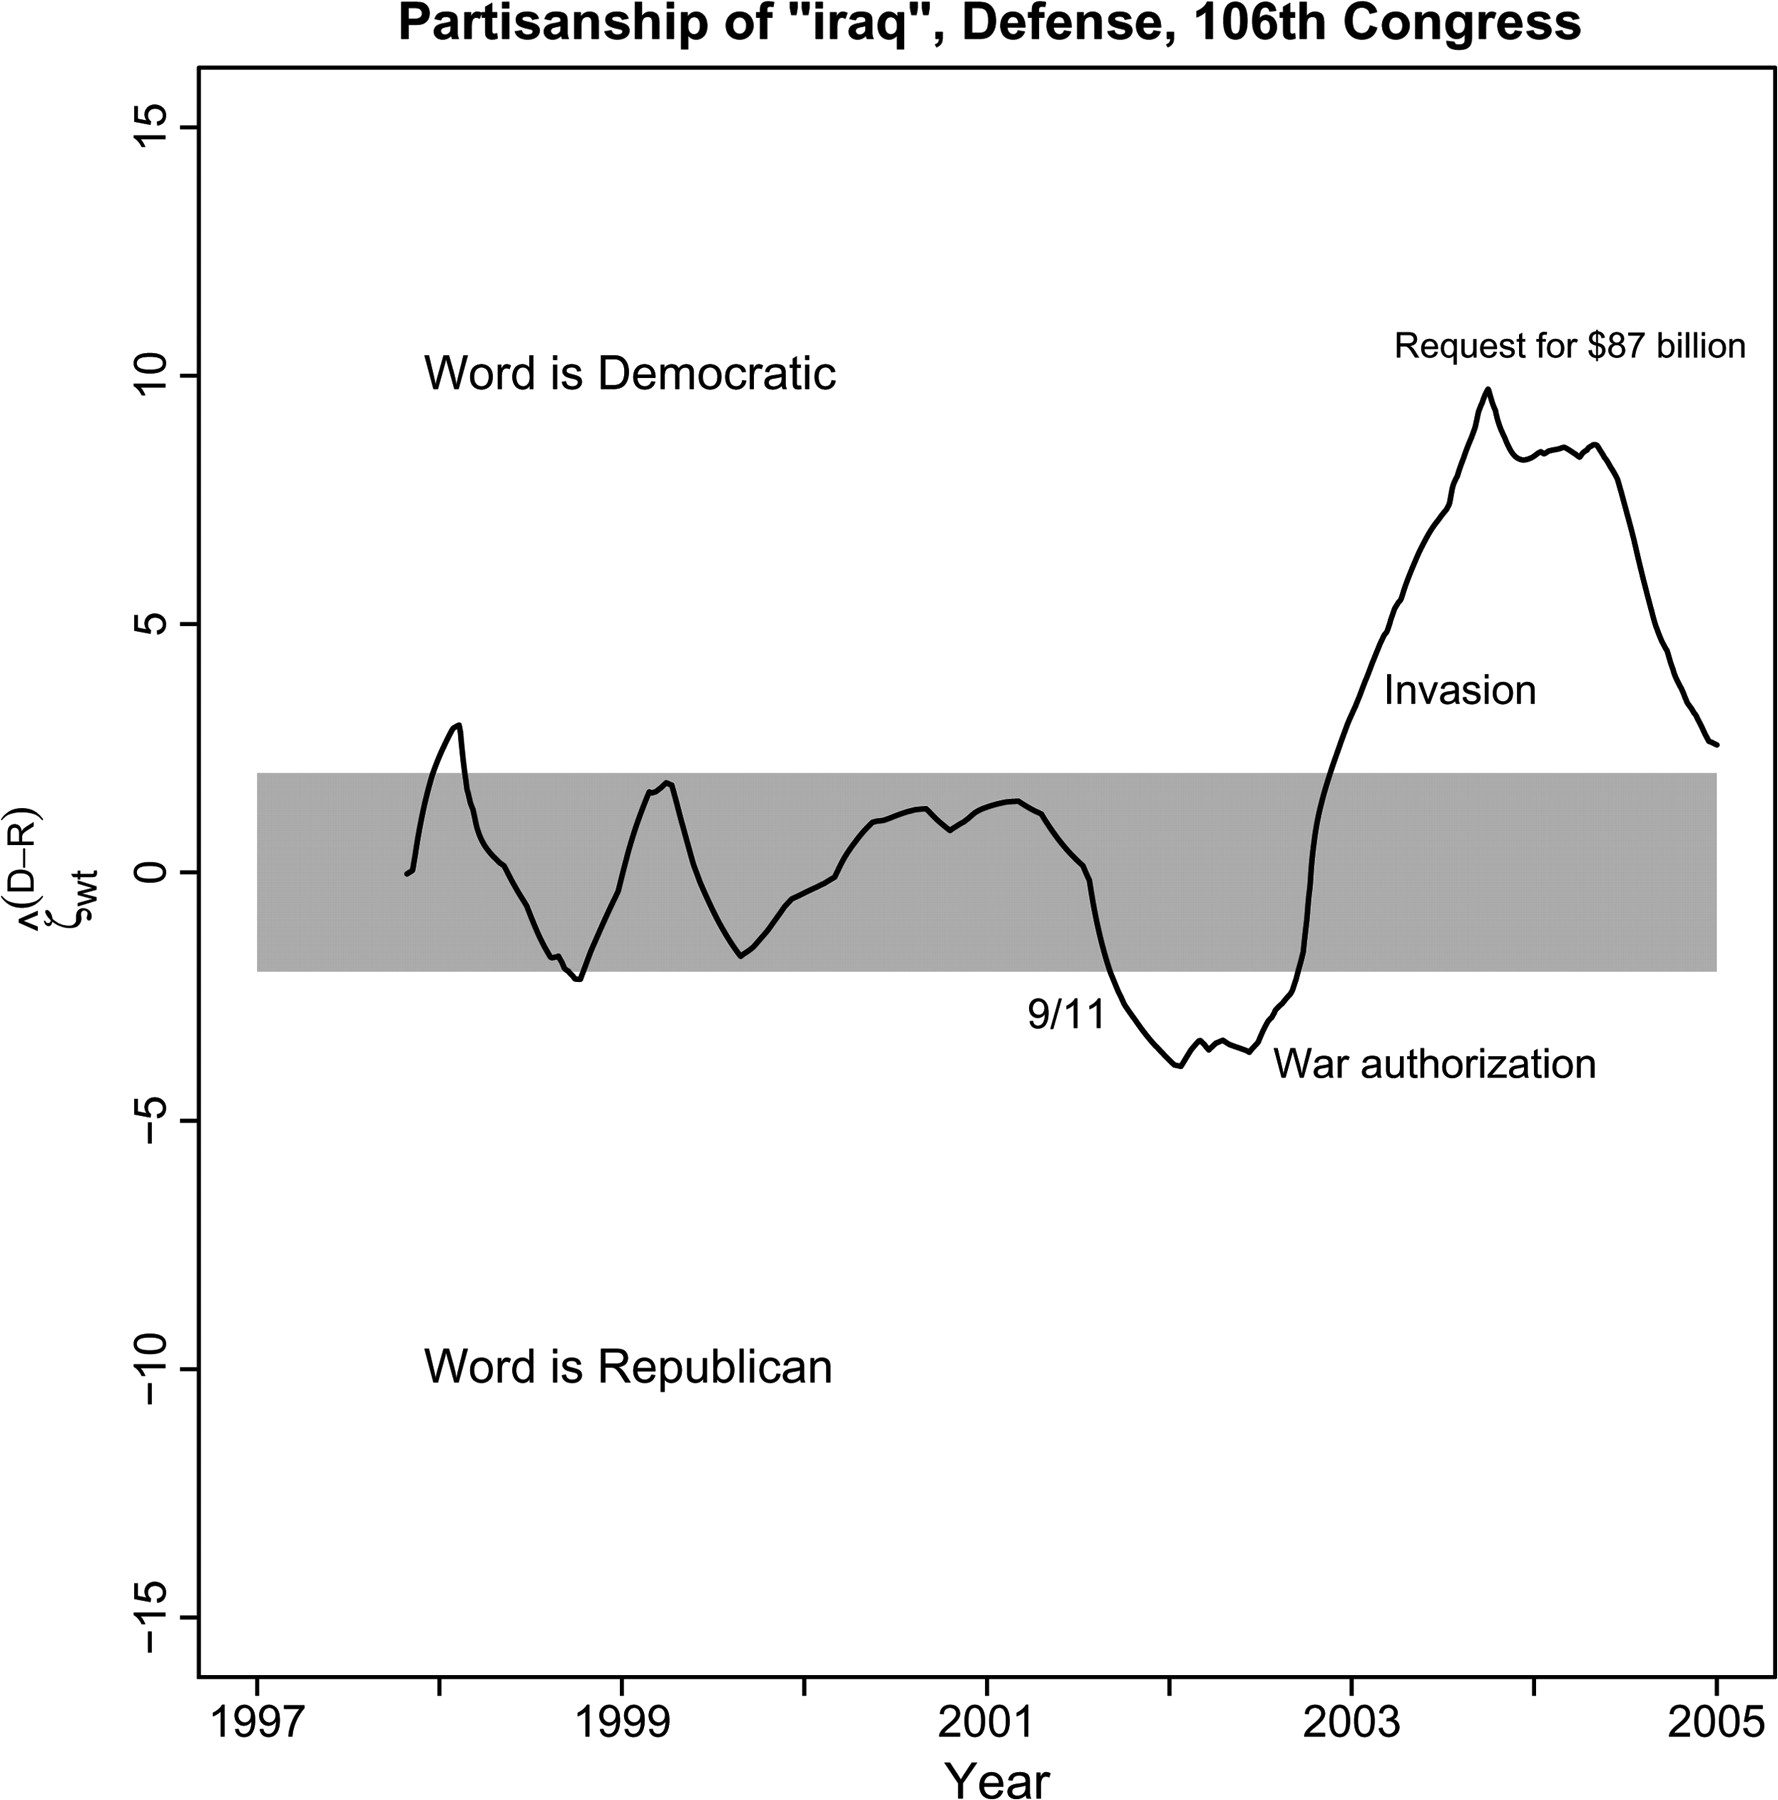
\includegraphics[scale=.105]{pictures/fightin2.png}
\end{figure}
\nocite{Monroe.etal2008}
\end{frame}

\begin{frame}{Algorithmic instability}

\begin{figure}[hbt]
  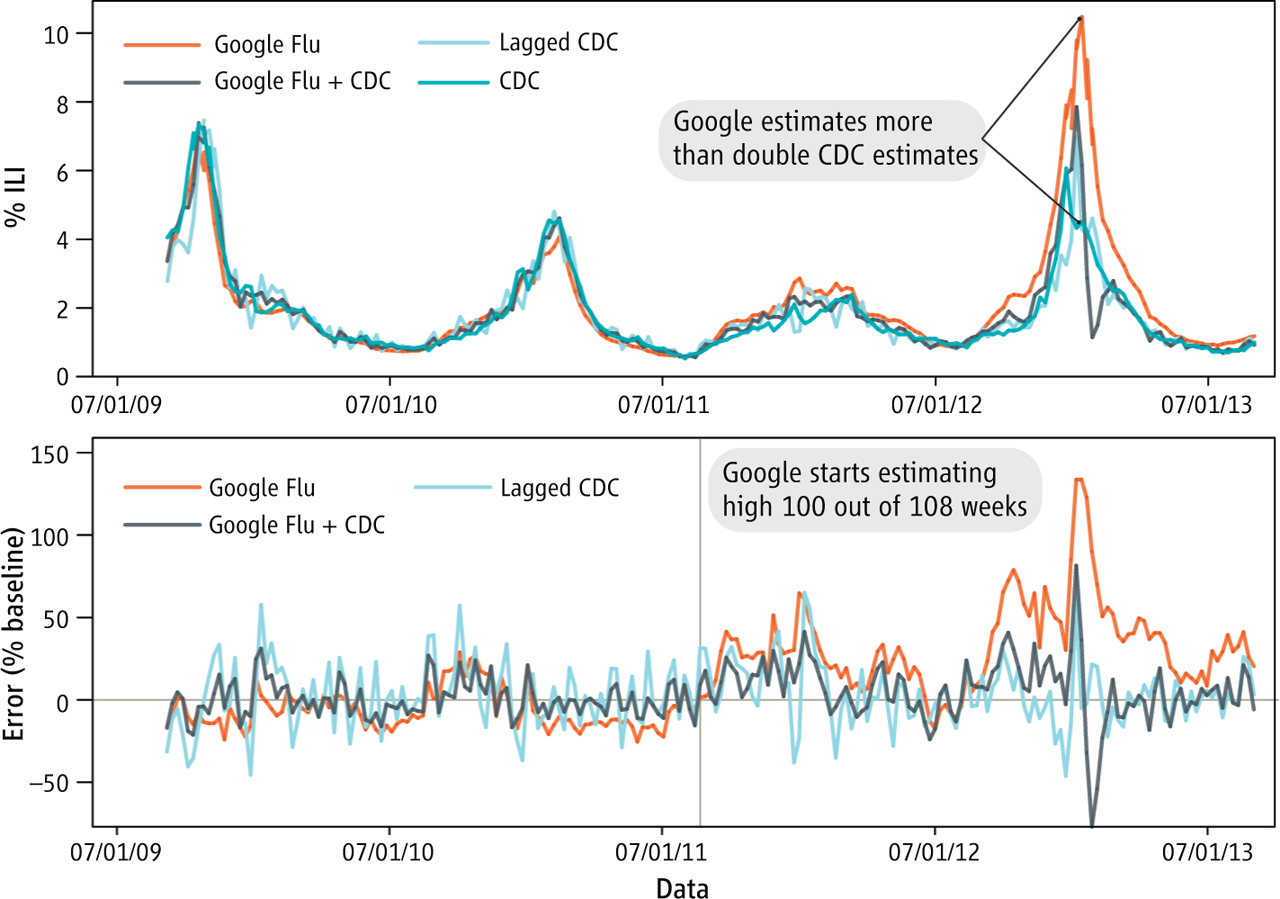
\includegraphics[scale=.9]{pictures/science-google-flu.jpg}
  \caption{\cite{Lazer.etal2014}}
\end{figure}
\end{frame}


\begin{frame}{Reflexive solutions}

Sometimes these actors are happy to solve comparability problems for us, e.g.
\begin{itemize}
  \item Lower court opinions \parencite{Corley.etal2011} or Amicus briefs \parencite{Collins.etal2015} \textit{embedded in} Supreme Court opinions
  \item ALEC model bills \textit{embedded in} state bills \parencite{Garrett.Jansa2015}
\end{itemize}

A perfect jobs for \textit{text-reuse} algorithms\ldots

\end{frame}

\begin{frame}{Communication: Randomness}

Why randomness?

You almost never \textit{say exactly the same words twice},
even when you haven't changed your mind about the message.

Hence words are the result of some kind of \textit{sampling process}.

We model this process as random because we don't know or care about
all the causes of variation (and because we're all secretly Bayesians)

Note: this is randomness \textit{conditional on the institution}

\end{frame}

{\setbeamertemplate{navigation symbols}{}
\begin{frame}
\vfill
\vspace{10ex}
\centerline{\Huge\color{gray}\decorativeflower}
\vfill
\end{frame}
}

\begin{frame}{Words as data}

What do we know about words as data?

They are \textit{difficult}
\begin{itemize}
  \item High dimensional
  \item Sparsely distributed (with skew)
  \item Not equally informative
\end{itemize}

\end{frame}

\begin{frame}{Difficult words}

Example: Conservative party 2017 manifesto compared to other parties over four elections:

\begin{itemize}
  \item \textit{High dimensional}.  3784 word types (adult native english speakers know ~20-35,000)
  \item \textit{Sparse}. Of 16083, word types in total, the Conservatives only used 3784
  \item \textit{Skewed}. Of these 1731 words appeared exactly once and the most frequent word 1757 times
\end{itemize}

\pause 
~\\
More generally: the Zipf-Mandelbrot law \parencite{Zipf1932,Mandelbrot1966}
$$
F(W_i) \propto 1/{\text{rank}(W_i)^\alpha}
$$
where $\text{rank}(.)$ is the
frequency \textit{rank} of a word in the vocabulary and
$\alpha\approx 1$

This is a Pareto distribution in disguise

\end{frame}


\begin{frame}{Difficult at all scales}




\begin{columns}[T,onlytextwidth]
\column{0.45\textwidth}

\centerline{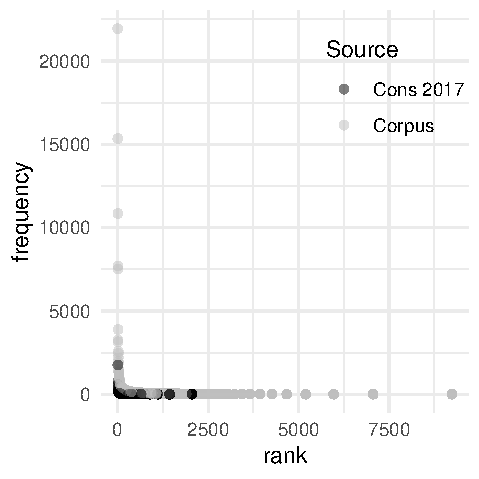
\includegraphics[scale=0.7]{figures/allscalesorig}}

%\column{0.1\textwidth}
\column{0.45\textwidth}

\centerline{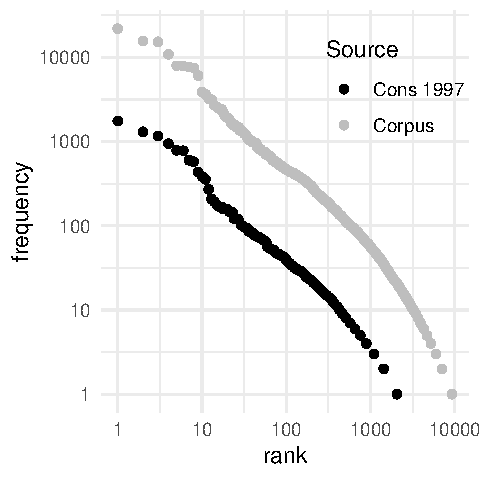
\includegraphics[scale=0.7]{figures/allscaleslog}}

\end{columns}

See \textcite{Chater.Brown1999} on scale invariance.

\end{frame}

\begin{frame}{Types and Tokens}

\begin{columns}[T,onlytextwidth]
\column{0.5\textwidth}

More generally: the Heaps-Herdan Law states that the number of
word types appearing for the first time after n tokens is
$$
D(n) = K n^\beta
$$
where $K$ is between 10 and 100 and $\beta \approx 0.5$ for English.

~\\

(All the party manifestos shown here)

\column{0.05\textwidth}
\column{0.45\textwidth}

\centerline{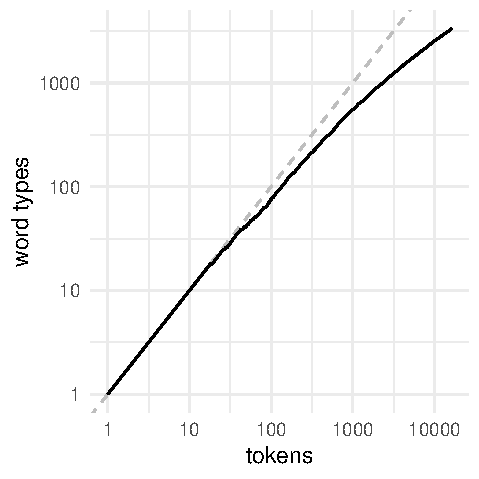
\includegraphics[scale=0.7]{figures/heaps}}

\end{columns}

\end{frame}


\begin{frame}{Frequency and interestingness}

Frequency is inversely proportional to substantive interestingness

~\\
\begin{columns}[T,onlytextwidth]
\column{0.33\textwidth}

\begin{center}
\begin{tabular}{rlr}
  \toprule
 & Word & Freq. \\ 
  \midrule
1 & the & 21939 \\ 
  2 & and & 15747 \\ 
  3 & to & 15347 \\ 
  4 & of & 10850 \\ 
  5 & we & 7943 \\ 
  6 & will & 7930 \\ 
   \bottomrule
\end{tabular}


~\\
Top 10
\end{center}
\column{0.33\textwidth}


\begin{center}

\begin{tabular}{rlr}
  \toprule
 & Word & Freq. \\ 
  \midrule
16078 & 1.83 & 1 \\ 
  16079 & 2.20 & 1 \\ 
  16080 & 1.35 & 1 \\ 
  16081 & 33.34 & 1 \\ 
  16082 & 1.71 & 1 \\ 
  16083 & rigination & 1 \\ 
   \bottomrule
\end{tabular}


~\\
Bottom ten
\end{center}

\column{0.33\textwidth}
\begin{center}
% latex table generated in R 4.0.2 by xtable 1.8-4 package
% Tue Sep  8 12:53:29 2020
\begin{table}[ht]
\centering
\begin{tabular}{rlr}
  \hline
 & Word & Freq. \\ 
  \hline
20 & people & 1929 \\ 
  26 & new & 1507 \\ 
  27 & government & 1493 \\ 
  33 & support & 1212 \\ 
  34 & work & 1143 \\ 
  36 & uk & 1058 \\ 
   \hline
\end{tabular}
\end{table}


~\\
Top ten minus \textit{stopwords}
\end{center}

\end{columns}

\end{frame}

\begin{frame}{Dealing with difficult words}

Removing stopwords, while standard in computer science, is not necessarily better\ldots

Example:
\begin{itemize}
\item Standard collections contain, `him', `his', `her' and `she'.
\item Words you'd want to keep when analyzing an abortion debates.
\end{itemize}

\end{frame}

\begin{frame}{Dealing with difficult words}

For large amounts of text summaries are not enough.

We need a \textit{model} to provide assumptions about
\begin{itemize}
  \item \textit{equivalence}
  \item \textit{exchangeability}
\end{itemize}


%Two words may
%\begin{tabular}{ll}
%\textsl{refer} to the same thing & (co-reference) \\
%\textsl{mean} the same thing & (synonymy) \\
%are \textsl{adjectives} & (syntactic role)\\
%\textsl{express} hostility, identity, \ldots & (pragmatics)\\
%\end{tabular}

Text as data started off making most use of equivalence, and ended up with increasingly sophisticated versions of exchangeability

Since ontogeny recapitulates phylogeny, let's walk through some standard text processing steps, asserting equivalences along the way\ldots

\end{frame}
\begin{frame}[t]\frametitle{Punctuation invariance}

\begin{quote}As I look ahead I am filled with foreboding.  Like the Roman I seem to see `the river Tiber flowing with much blood'\ldots ''\\
\hfill\parencite{Powell1968}
\end{quote}

\pause

\begin{center}
{\small
\begin{tabular}{ll}\toprule
index & token\\ \midrule
1 & as\\
2 & i\\
3 & look\\
4 & ahead\\
5 & i\\
6 & am\\
7 & \ldots\\ \bottomrule
\end{tabular}
~~~~~~~~~~
\begin{tabular}{ll}\toprule
index & token\\ \midrule
1 & like\\
2 & the\\
3 & roman\\
4 & i\\
5 & seem\\
6 & to\\
7 & \ldots\\ \bottomrule
\end{tabular}
}
\end{center}


\end{frame}
\begin{frame}[t]\frametitle{Lexical univocality}

\begin{center}
{\small
\begin{tabular}{ll}\toprule
type & count\\ \midrule
as & 1\\
i & 2\\
look & 1\\
ahead & 1\\
am & 1\\
\ldots & \ldots\\ \bottomrule
\end{tabular}
~~~~~~~~~~
\begin{tabular}{ll}\toprule
token & count\\ \midrule
like & 1\\
the & 1\\
roman & 1\\
i & 1\\
seem & 1\\
to & 1\\
\ldots & \ldots\\ \bottomrule
\end{tabular}
}
\end{center}

\end{frame}
\begin{frame}[t]\frametitle{Order invariance}

\begin{center}
{\small
\begin{tabular}{rlll}\toprule
&         & unit    & \\ \midrule
&         & `doc' 1 & `doc' 2 \\ \midrule
type      & ahead   & 1    & 0 \\
& am      & 1    & 0 \\
& as      & 1    & 0 \\
& i       & 2    & 1 \\
& like    & 0    & 1\\
& look    & 1    & 0 \\
& roman   & 0    & 1 \\
& seem    & 0    & 1 \\
& the     & 0    & 1 \\
& to      & 0    & 1\\
& \ldots  & \ldots & \ldots \\ \bottomrule
\end{tabular}
}
\end{center}

\end{frame}

\begin{frame}[t]\frametitle{Count data}

We have turned a corpus into a \textit{contingency table}.
\begin{itemize}
\item Or a term-document / document-term / document-feature matrix, in the lingo
\end{itemize}

~\\
Everything you learned in your categorical data analysis course applies
\begin{itemize}
\item except that the variables of interest: $\theta$ are \textit{not observed}
\end{itemize}

%%%%%%%%%%%

\end{frame}
\begin{frame}[t]\frametitle{Count data}

We have turned a corpus into a \textit{contingency table}.
\begin{itemize}
\item Or a term-document / document-term / document-feature matrix, in the lingo
\end{itemize}

\begin{center}
{\small
\begin{tabular}{rllllllllll}\toprule
      & ahead & am & i & like & look & & \\ \midrule
doc 1 & 1     & 1  & 2 & 0    & 1    & \ldots & \textcolor{gray}{$\theta_{doc1}$} \\
doc 2 & 0     & 0  & 1 & 1    & 0    & \ldots & \textcolor{gray}{$\theta_\text{doc2}$} \\ \midrule
      & \textcolor{gray}{$\beta_\text{ahead}$}
      & \textcolor{gray}{$\beta_\text{am}$}
      & \textcolor{gray}{$\beta_\text{i}$}
      & \textcolor{gray}{$\beta_\text{like}$}
      & \textcolor{gray}{$\beta_\text{look}$} \\ \bottomrule
\end{tabular}
}
\end{center}


Everything you learned in your categorical data analysis course applies
\begin{itemize}
\item except that the variables of interest: $\theta$ are \textit{not observed}
\end{itemize}
What are we going to assume about the cell contents?

%%%%%%%%%%%

\end{frame}
\begin{frame}{Statistical assumptions about words}

Word counts/rates are conditionally \textit{Poisson}:
$$
W_j ~\sim~ \text{Poisson}(\textcolor{black}{\lambda_{j}})
$$
Curiously
$$
\ex[W]  ~=~ \text{Var}[W] ~=~ \lambda
$$

Rate models are naturally \textit{multiplicative}.
\begin{itemize}
  \item Rates increase / decrease by X\%
\end{itemize}

Model assumptions are will turn on how $\lambda$ is
related to $\theta$

\end{frame}

%## Statistical assumptions about words
%
%%## Statistical models of words: Poisson
%
%```{r, out.width="80%"}
%knitr::include_graphics("pictures/geiger-counter.jpg")
%```
%

\begin{frame}{Statistical assumptions about words}

That means that for fixed document lengths, counts are conditionally \textit{Multinomial}:
$$
W_{i1}\ldots W_{iV} ~\sim~ \text{Mult}(W_{i1}\ldots W_{iV} \mid \textcolor{black}{\pi_{1}}\ldots\textcolor{black}{\pi_{V}}, N_i)
$$
Here
$$
\ex[W] = N\pi
$$
and
$$
\text{Cov}[W_{i}, W_{j}] = -N \pi_{i}\pi_{j}
$$

Negative covariance is due to the `budget constraint'
\end{frame}

\begin{frame}\frametitle{Modelling decisions}

For each research problem involving content analysis we need to ask:
\begin{itemize}
\item What \textit{structure} does $\theta$ have
\item What counts as a \textit{word}?
\item What counts as a \textit{document}?
\item What is \textit{observed}, what is \textit{assumed}, and what is \textit{inferred}?
\item What is the \textit{relationship} is between $\theta$ and the words? The model
\end{itemize}

\end{frame}


\begin{frame}{The space of models}

\centerline{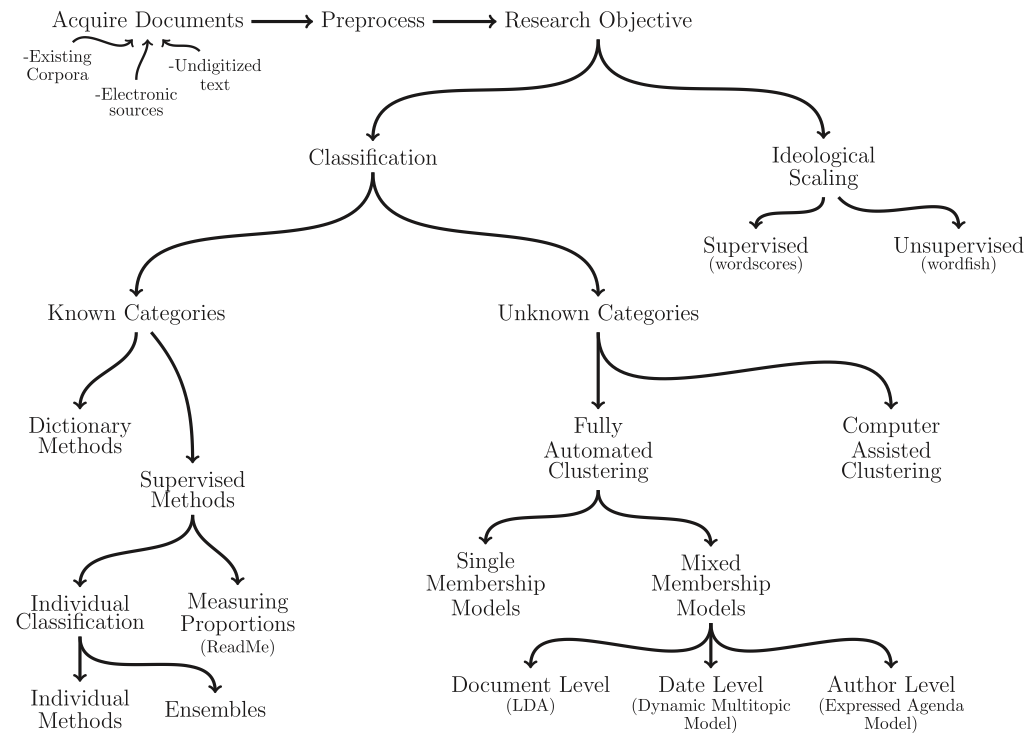
\includegraphics[scale=0.25]{pictures/tad-picture.png}}

\end{frame}

\begin{frame}{In the general measurement problem}

\centerline{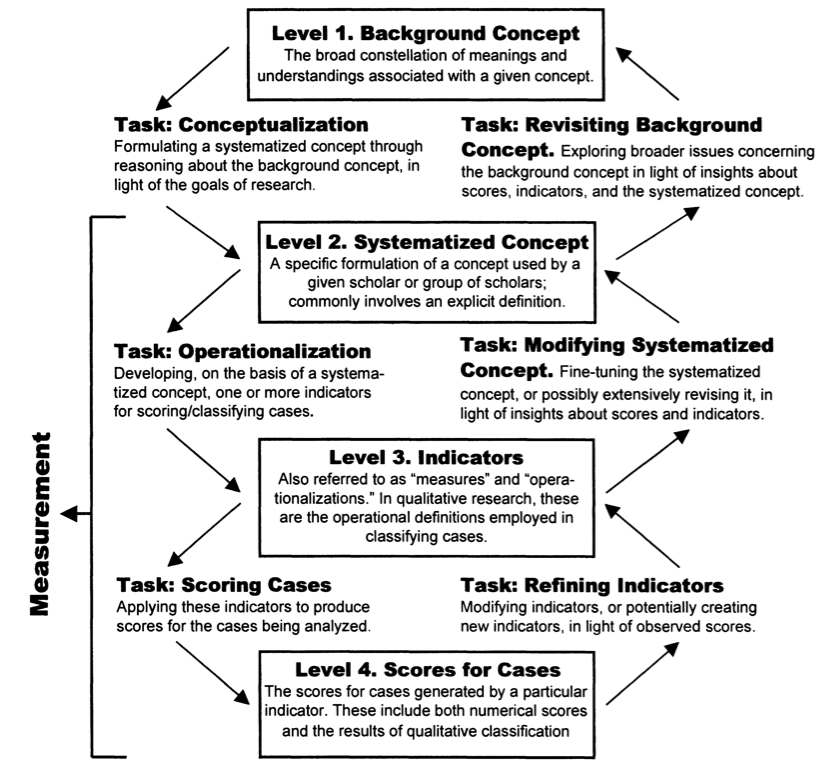
\includegraphics[scale=0.25]{pictures/measurement-validity.png}}

\end{frame}


{\setbeamertemplate{navigation symbols}{}
    \begin{frame}{}
      \vfill
      \vspace{10ex}
      \centerline{\color{gray}\Huge\decorativeflower}
      \vfill
    \end{frame}
}

\begin{frame}{Exchangeability and the `bag of words'}

~\\
\centerline{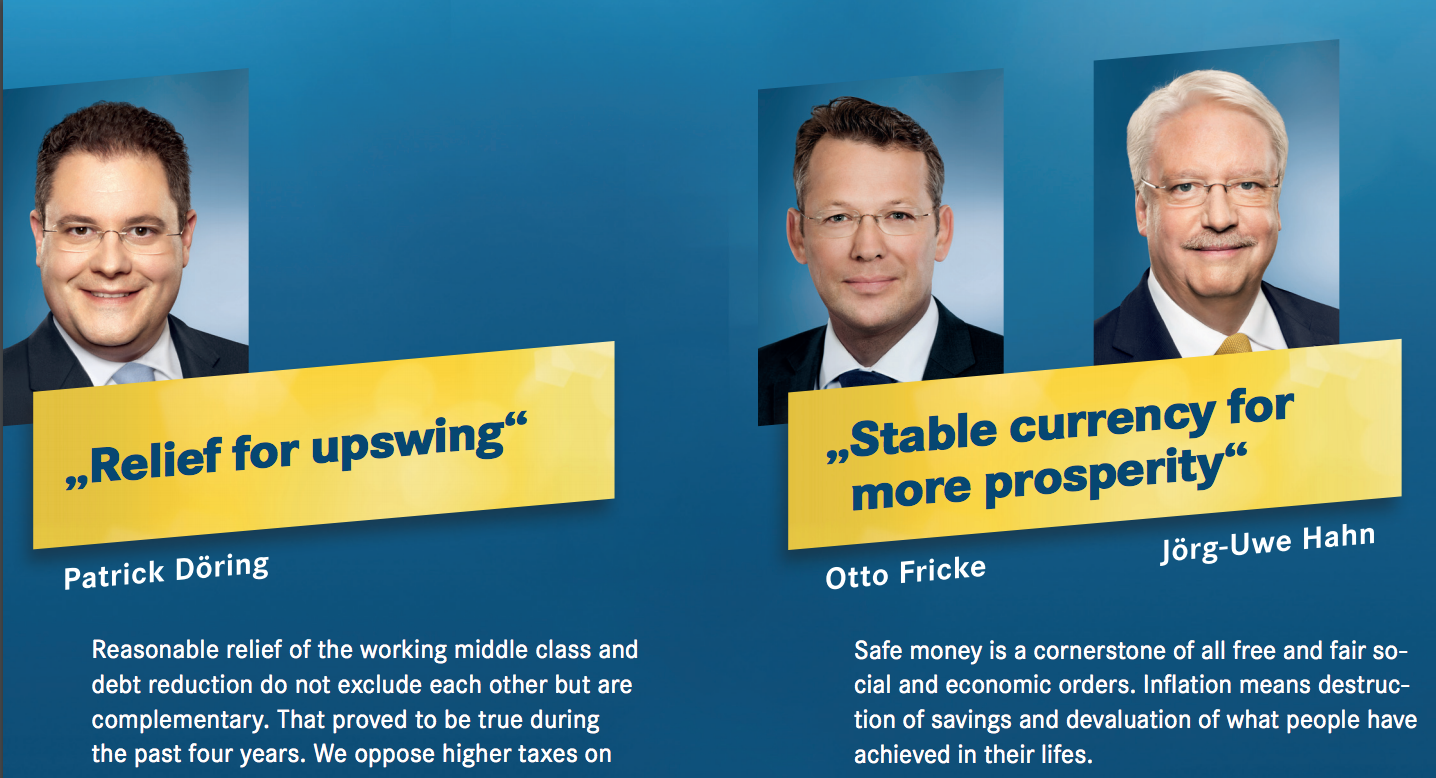
\includegraphics[scale=0.4]{pictures/fdp-en.png}}

\end{frame}

\begin{frame}{The marginal challenge}

The original:

~\\
\begin{quote}
Reasonable relief of the working middle class and
debt reduction do not exclude each other but are
complementary. That proved to be true during
the past four years. We oppose higher taxes on
citizens and businesses. They prevent growth and
kill jobs, thus putting at risk the very existence of
countless workers and their families.
\end{quote}


Given the \textit{marginal distribution of word types} a.k.a. the `bag of words' how different could the meaning of the resulting document be?

\end{frame}

\begin{frame}{Slightly different...}

A possible reconstruction

~\\
\begin{quote}
We oppose higher taxes because they prevent growth and
kill jobs, risking the very existence of
countless families and businesses. Debt reduction is
complementary to reasonable relief of the
working middle class; they do not exclude each other.
That proved to be true in the last four years.
\end{quote}

But much the same sense

\end{frame}
\begin{frame}{Looser constraints}

We can make this a more semantic challenge by only demanding
the substantically interesting word margins are maintained.

~\\
\begin{quote}
businesses reasonable existence countless
reduction families prevent risking working exclude oppose
higher growth relief middle proved taxes class years kill
jobs debt true last four complementary
\end{quote}

Removing stopwords mostly just removes \textit{grammatical} constraints

~\\
To the extent this set of words characterizes what the FDP wanted to express in their platform, the `bag of words' assumption is reasonable.

\end{frame}

\begin{frame}{But negation!}


If we can add grammatical functors at will, could we
make the opposite meaning by negating everything?

In principle (and in practice for some discursive forms) yes, yes we could.

And the bag of words assumption would fail

\pause

An interesting \textit{empirical fact} about political discourse is that
actors do not tend to disagree by negation but by redirection or
diversion.
\begin{itemize}
  \item Simple version: You talk about the environment, I talk about economic growth
  \item Sophisticated version: The `heresthetic' \parencite{Riker.etal1996}
\end{itemize}

\end{frame}


\begin{frame}{Exchangeability and the `bag of words'}
	
Technically a sequence of random variables is \textit{exchangeable} if 
their \textit{joint probability distribution} is invariant to reordering them
\begin{itemize}
  \item a `weaker' relationship than identical and independently distributed (iid)
\end{itemize}

\textcite{deFinetti2008} showed that if we assume $\{W_i\}$ are exchangeable, then this is equivalent to assuming that they are (loosely speaking) generated by a distribution parameterize dby some $\theta$:
$$
P(W_1 \ldots W_V) = \int \prod^V_v P(W_v \mid \theta) P(\theta) d\theta 
$$
This is `the Representation Theorem' and motivates our measurement model assumptions earlier

\begin{center}
\begin{tikzpicture}
\node(pre) at (0,   0) [var]{};
\node(W1) at  (1, 0)[var]{};
\node(W2) at  (2,   0) [var]{};
\node(W3) at  (3, 0) [var]{};
\node(theta) at (2,1)  [lat,label=above:$\theta$]{};
\node(post) at (4, 0) [var]{};
\draw  (theta) -- (pre);
\draw  (theta) -- (W1);
\draw  (theta) -- (W2);
\draw  (theta) -- (W3);
\draw  (theta) -- (post);
\end{tikzpicture}
\end{center}
\end{frame}


\begin{frame}{}
\end{frame}



%%%%%%%%%%%%%%%%%%%%%%%%%%

\begin{frame}[allowframebreaks]
\frametitle{References}

\printbibliography

\end{frame}

\end{document}





%
%## Labs
%
%```{r, out.width = "80%", fig.cap = "'You must press the button. I'm a scientist you know!'"}
%knitr::include_graphics("pictures/milgram-machine.jpg")
%```
%
%## Menu
%
%**Session 1: How could this possibly work?**
%
%Session 2: Dictionary-based 'classical' content analysis and topic models
%
%Session 3: Scaling models
%
%Session 4: Getting hold of the data
%
%## Focus
%
%Assumptions
%
%Interpretation
%
%Justification
%
%Pitfalls
%
%Mechanics (in Lab)
%
%##
%
%```{r, out.width = '80%'}
%knitr::include_graphics("pictures/etinarcadiaego.jpg")
%```
%
%


%
%```{r, out.width = '90%'}
%knitr::include_graphics("pictures/grey-just-rile.pdf")
%```
%
%## Statistical assumptions about words
%
%Word counts/rates are conditionally Poisson:
%$$
%W_j ~\sim~ \text{Poisson}(\textcolor{red}{\lambda_{j}})
%$$
%
%Expected $W_{j}$ (and its variance) is $\lambda_{j}$
%
%Models are naturally *multiplicative*. Rates increase by
%10%, decrease by 20%
%
%. . .
%
%The rate $\lambda$ depends on $\theta$ in a more or less complex fashion.
%
%## Statistical models of words: Poisson
%
%```{r, out.width="80%"}
%knitr::include_graphics("pictures/geiger-counter.jpg")
%```
%
%## Statistical models of words: Multinomial
%
%For *fixed* document lengths, counts are conditionally Multinomial:
%$$
%W_{1}\ldots W_{V} ~\sim~ \text{Multinomial}(W_{1}\ldots W_{V} \mid \textcolor{red}{\pi_{1}}\ldots\textcolor{red}{\pi_{V}}, N_i)
%$$
%
%Expected $W_{i}$ is $N\pi_{i}$
%
%Covariance of $W_{i}$ and $W_{j}$ is $-N \pi_{i}\pi_{j}$
%
%Negative covariance is due to the 'budget constraint'
%
%## Statistical models of words: Multinomial
%
%```{r, out.width = '80%'}
%knitr::include_graphics("pictures/20-sided-die.jpg")
%```
%## Implication: Absence is an observation
%
%Note: Don't be fooled...
%
% - Statistical models of text deal with *absence* as well as presence:
%   zeros count
% - Absence is informative *to the extent it is surprising*
% - Surprise implies expectations; expectations imply a model.
%
%
%## Exchangeability and the 'bag of words'
%
%```{r, out.width = '90%'}
%knitr::include_graphics("pictures/fdp-en.png")
%```
%
%## Intuition: the marginal challenge
%
%The original:
%
%> Reasonable relief of the working middle class and
%> debt reduction do not exclude each other but are
%> complementary. That proved to be true during
%> the past four years. We oppose higher taxes on
%> citizens and businesses. They prevent growth and
%> kill jobs, thus putting at risk the very existence of
%> countless workers and their families.
%
%. . .
%
%Given the *marginal distribution of word types* here a.k.a. the 'bag of words' and
%a long afternoon...
%
%- Just how different could the meaning of the resulting document be?
%
%
%## Slightly different...
%
%A possible reconstruction
%
%> We oppose higher taxes because they prevent growth and
%> kill jobs, risking the very existence of
%> countless families and businesses. Debt reduction is
%> complementary to reasonable relief of the
%> working middle class; they do not exclude each other.
%> That proved to be true in the last four years.
%
%But much the same sense
%
%## Looser constraints
%
%We can make this a more semantic challenge by only demanding
%the substantically interesting word margins are maintained.
%
%> businesses reasonable existence countless
%> reduction families prevent risking working exclude oppose
%> higher growth relief middle proved taxes class years kill
%> jobs debt true last four complementary
%
%(Removing stopwords mostly just removes *grammatical* constraints)
%
%## But negation!
%
%Wait, if we can add grammatical functors at will, could we
%make the opposite meaning by negating everything?
%
%. . .
%
%In principle (and in practice for some discursive forms) yes, yes we could.
%And the bag of words assumption would fail
%
%. . .
%
%An interesting *empirical fact* about political discourse is that
%actors do not tend to disagree by negation but by redirection or
%diversion.
%
%- Simple version: You talk about the environment, I talk about economic growth
%- Sophisticated version: The 'heresthetic' [@Riker.etal1996]
%
%## What is this content $\theta$?
%
%What is the content in content analysis?
%
% - Documents are *mixtures of categories*: policy agenda of a speech
% - Documents have *categories*: topic of a press release
% - Documents have *positions*: ideological position of a legal brief
%
%Important things we will not discuss:
%
% - Documents as collections of facts and assertions
% - Documents as networks
%
%## Specifically: NLP
%
%'Natural Language Processing' (NLP) tasks, some of which
%may be of use to us:
%
%- Segmentation / Tokenization: Finding where the words and sentences are
%- Lemmatization: Stripping a word down to its 'root'
%- Part of Speech (POS) tagging: Associating grammatical
%  roles with words (noun, verb, determiner, preposition, etc.)
%- Parsing: Associating grammatical structures with sentences
%  (typically dependency graphs, but sometimes trees and
%  feature structures)
%
%
%## Specifically: NLP
%
%- Named Entity Recognition (NER): Identifying people, places, and things
%- Information Extraction (IE): Extracting 'facts' (who did
%  what to whom, when)
%
%. . .
%
%Tools:
%
%- [Spacy](https://spacy.io) (Python) via `{spacyr}`,
%  [Stanford NLP tools](https://nlp.stanford.edu/software/),
%  (Java) via `{CoreNLP}` (or `{cleanNLP}` which wraps both).
%  Also [OpenNLP](http://opennlp.apache.org/) (Java) via
%  `{openNLP}`.
%
%## What is this content $\theta$?
%
%```{r, out.width="80%"}
%knitr::include_graphics("pictures/tad-picture.png")
%```
%
%## What is this content $\theta$?
%
%```{r, out.width="80%"}
%knitr::include_graphics("pictures/measurement-validity.png")
%```
%
%## Commitment anxiety
%
%What more are we committing to in this quantitative content analysis
%framework?
%
%- substantive theory $\neq$ textual measurement
%
%but they do have implications for one another
%
%## A Theory/measurement distinction
%
%Discourse analysis tends to *tightly couple* theory and measurement
%
%\footnotesize
%**A complete package**
%
%Although discourse analysis can be applied to all areas of
%research, it cannot be used with all kinds of theoretical
%framework. Crucially, it is not to be used as a method of
%analysis detached from its theoretical and methodological
%foundations. Each approach to discourse analysis that
%we present is not just a method for data analysis, but a
%theoretical and methodological whole - a complete package.
%[...] In discourse and analysis theory and method are
%intertwined and researchers must accept the basic
%philosophical premises in order to use discourse analysis as
%their method of empirical study.
%\normalsize
%
%[@Jorgensen.Phillips2002]
%
%## Not that
%
%. . .
%We will try as far as possible to separate theory and
%measurement (and concentrate on the second).
%
% - Our concerns: validity, stability
% - Rely on: transparency, reliability, replicability
%
%
%## The 'digital trace'
%
%\footnotesize
%
%"[J]ust as the invention of the telescope revolutionized the study of the heavens, so too by rendering the unmeasurable measurable, the technological revolution in mobile, Web, and Internet communications has the potential to revolutionize our understanding of ourselves and how we interact . [T]hree hundred years after Alexander Pope argued that the proper study of mankind should lie not in the heavens but in ourselves, we have finally found our telescope. Let the revolution begin."
%
%Duncan Watts (2011)
%\normalsize
%
%. . .
%
%The stars do not look differently when people are watching them.
%But our Instagram accounts do.
%
%## The 'digital trace'
%
%(or less romantically 'digital exhaust')
%
%In the worst case, our texts are
%
%- non-representative (all this guy does is eat)
%- incomplete (never sleeps)
%- positivity biased (but often pets puppies)
%- algorithmically confounded (and I see him everywhere)
%- ethically challenging (so I downloaded all his posts)
%
%. . .
%
%Just like most other kinds of data about people in the
%social sciences...
%
%
%
%## Lab time
%
%```{r, out.width = '90%'}
%knitr::include_graphics("pictures/hieroglyphic-keyboard-cm.jpg")
%```
%## References  {.allowframebreaks}
%
%\tiny

